\documentclass[12pt]{article}
\usepackage[english]{babel}
\usepackage[utf8]{inputenc}
\usepackage{blindtext, fancyhdr}
\usepackage{graphicx}
\usepackage{amsmath}
\usepackage{url}
\emergencystretch=1em
\pagestyle{fancy}

\title{Cut Detection Survey and Analysis for Long Form Video Game Streams \\ Prof. Prosenjit Bose}
\author{Jaime Herzog\\ 101009321 \\ jaimeherzog@cmail.carleton.ca}

\fancyhf{}
\rhead{\textit{\rightmark}}
\lhead{\textit{\leftmark}}
\rfoot{\thepage}

\begin{document}

\maketitle
\clearpage

\section{Abstract}
Shot Boundary Detection, or simply Shot Detection, is a fundamental part of research in the broader field of video analytics, used for essential video analysis tasks such as 
video indexing and content-based video retrieval. For professional video game live streamers, who create hours of continuous content with significant downtime, identifying
cuts in their streams is an important first step for automatically generating condensed stream highlights. In this project, I have summarized the nomenclature and methodologies
established in the academic canon for Cut Detection research, implemented a sample of the most common approaches, Colour Histogram comparison and Edge Change Ratio using Canny 
Edge Detection, and compared their effectiveness when used on video game live stream content, as well as establishing methodological challenges to this new content form.
\section{Acknowledgements}
Thank you to my project supervisor Professor Prosenjit Bose for his help and direction throughout this project.
\clearpage

\tableofcontents
\clearpage

\listoffigures
\listoftables
\clearpage

\section{Motivation}
\subsection{Why Shot Boundary Detection?}
    With the proliferation of internet connectivity in recent years, there has been a massive increase in the volume of video on the internet.
With this growth, an industry built around the creation, hosting and sharing of video content grew as well, with YouTube alone having an annual revenue of over US\$15 billion
dollars~\cite{youtube}. Portable devices increase the accessibility for the creation and uploading of video content, and the combination of the 
massive social network surrounding content creation, with the enticing entertainment industry creating multi-millionaire content creators has 
exploded the sheer hours of video being uploaded daily. For YouTube, this type of content tends towards short-form video content at an average of about 10 minutes long. Comparing
this to video game live streamers, who in some cases are live 8 hours a day, 5 days a week, with some streaming even more frequently, the volume of video uploaded
per creator is significantly increased. In Q4 2019, there were 2.3 billion hours watched on Twitch, and 0.9 billion on YouTube Gaming~\cite{twitchusage}. 

    For live streamers, when they have so much continuous uptime, it is important to create highlights of their daily streams, in order to increase their reach to viewers who
don't have the time to watch their full time streams, as well as to diversify their brand onto a traditional YouTube channel. The creation of these highlights is extremely
time consuming, as the hours of content must be sifted through manually by either the content creators themselves, adding hours to their daily workload, or by hired editors. 
Commonly, it is unfeasable for streamers to spend all their spare time manually editing highlight videos for their daily streams, and for streamers with a lower viewerbase
and thus less income, it is also difficult to afford a full time editor. This creates another barrier of entry to the career of live streaming, a career track that is already
difficult to get started in due to the high viewership required for career viability. The solution for this currently manual labour is an automated editing system, which 
methodologically identifies key scenes and removes downtime. This could use some implementation of technology analogous to Story Segmentation, which was a task for TRECVID 2003
~\cite{storyseg}, or using representative key frame extraction. However, for anything like Story Segmentation or key frame extraction to be possible, it is essential that the
system first defines the video's scenes. To do this, we must find where begin and end, hence we use various shot boundary detection methods. 

\subsection{Cut Detection and Video Game Live Streaming}
    There has been siginificant research in the field of shot boundary detection over the past couple of decades, with multiple surveys of traditional shot detection methods
~\cite{lienhart1998comparison}~\cite{survey1}. Shot boundary detection is a fundamental part of the broader field of video segmentation, which refers to the partitioning 
of video into spatial, temporal, or spatiotemporal regions that are homogeneous in some feature space. Video segmentation itself is an essential part of many video analysis problems,
including video summarization, indexing, retrieval, coding, authoring, and editing, as well as other applications in video surveillance and 3D motion ~\cite{bovik2009essential}. There are many different aspects of the shot boundary detection problem, due to the fact that shot boundary's can be defined by multiple 
different types of scene transitions - either an abrupt cut, or a gradual transition, such as a fade or a dissolve. These different transitions have different properties and patterns 
(see figure 1) that the shot boundary detection system must analyze, usually with each type of transition analyzed independently. For the purposes of this project, we will implement
systems which detect abrupt cuts in video, and then apply these to systems to video game live stream clips.
\begin{figure}[ht]
    \centering
    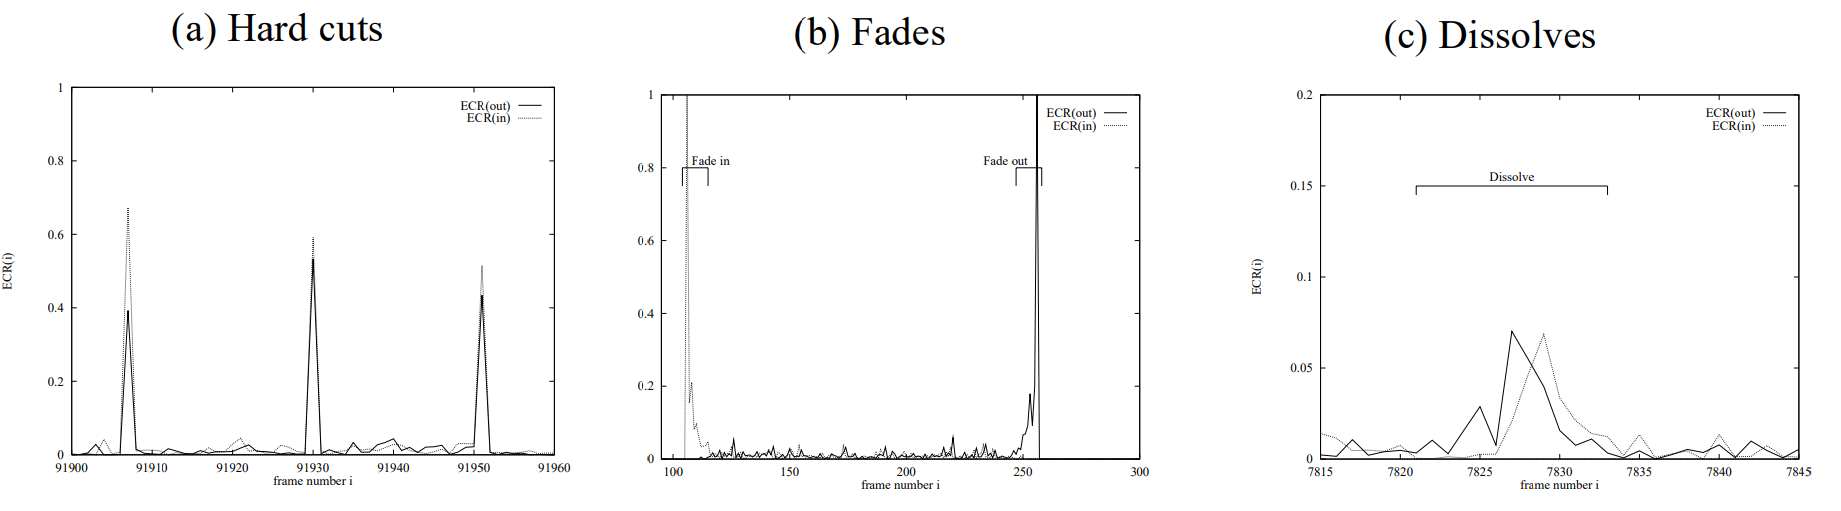
\includegraphics[width=1.0\textwidth]{fig1}
    \caption{Gradual Transitions: Their Differing ECR Values~\cite{lienhart1998comparison}}
    \label{Gradual Transitions}
\end{figure}

    Additionally, there has been as far as I know at the time of this project, limited ~\cite{ringer2018deep} research on the topic of video game live stream cut detection. It is understandable why - the 
video game live streaming industry is still very young, and the change in domain when compared to more typical edited video or film is significant. Rather than there being a typical 
film or video editor defining the end of each scene, we must analyze and formulate the typical "scenes" that define contiguous activity in video game live streams. 
This project will examine the different possible approaches to defining scenes in video game live streams, and attempt to formulate a schema for which we can apply 
traditional cut detection techniques, as well as outline areas of potential new developments for specifically this area, similar to what has been done for sports television
video segmentation.
\clearpage

\section{Methodology}
\subsection{What is Video Game Live Streaming?}
Video game live streaming is the activity of a person recording themselves playing a game to a live audience. Popularized in the mid 2010s primarily on Twitch, it started
as just people who enjoyed playing games playing for people to build an audience and have fun playing games. By 2014, Twitch had more traffic than HBO's online streaming 
service~\cite{graziano_2014}, and it had begun to become more and more clear that the popularity of these live streams could generate significant revenue. As the community grew,
so did avenues of revenue for streamers, and before long there were more than a handful of video game livestreamers generating significant income, with many more able to make a 
living off of streaming full time.



Currently, the profession of video game live streaming is appealing to many, but ultimately extremely inaccessable. This is due to the fact that a streamer must have an 
established and loyal community which supports the streamer with paid subscriptions through Twitch, donations, or via Patreon. Other sources of revenue include:
\begin{itemize}
    \item Salaries from esports teams such as Cloud 9 or TSM, although these sponsorships are reserved for the most popular or skilled streamers. 
    \item YouTube channels which host short form highlight videos. The problem with this was touched upon in the Motivation section, but to emphasize, 
    it is very time consuming for streamers to manually curate highlights and create entertaining videos on top of streaming consistent hours to grow their 
    community, and for new streamers who have jobs on top of their streaming, this becomes an insurmountable barrier of entry.
    \item Sponsored content, such as a game studio paying a streamer to play their game. Again, this type of revenue is only available to those select streamers
    who already have an established audience, as the paid content must be a viable investment to the sponsors.
\end{itemize}
This means that when a streamer is starting out, they must minimize their hours and keep a full time job, as it can take months or years before streaming 
income becomes viable full time. This leaves even less time for editing highlights of streams for increased reach, which further limits the accessibility
of building the brand necessary to be successful as a professional live streamer,  as discussed in the Motivation section.

\subsection{What is Shot Boundary Detection?}
We will begin by summarizing the problem of Shot Boundary Detection, and then we will take an overview of the formal schema for this problem as defined in ~\cite{survey1}
and how they must be modified to fit into the video game live stream content format.

Shot Boundary Detection is the problem of how to automatically detect the beginning or end of a shot or scene, which for traditional 
film would be defined more precisely as an uninterrupted sequence of images captured by a single camera action. 
While the number of possible types of scene transitions is quite large, in practice, the vast majority of all transitions are either hard cuts, fades,
or dissolves (at least when it comes to traditionally edited movies or video). 

\subsubsection{Defining a Cut in Video Game Live Streams}
We will now define what we will use as cuts in Video Game Live Streams between two categories:
\begin{enumerate}
    \item Scene transitions initiated by the streamer themselves, such as when they are transitioning from a full face camera to a game, or from game to game. Generally, 
    these are specially made transitions that match the streamer's branded overlay, and typically are fades or dissolves. Since these cover the whole screen and are 
    similar in structure to conventional dissolves or fades in film, we will not be focusing on these types of transitions in this project.
    \item Game transitions, i.e. transitions between different camera states in the game. Generally, in video games, there are three main camera states:
    \begin{enumerate}
        \item Menus. Players begin the game on a menu called the main menu, where they select one of various options, then start the gameplay. Typically, the main menu
        is a simple straight up view of a series of possible selections. These views tend to be relatively static and are rarely areas of concern for false positives for 
        any robust cut detection algorithm.
        \item Gameplay. When players make their selection on the main menu, the game begins, which typically involves the camera shifting from the static menu display to a 
        view of the player themselves. This view can have many different perspectives, but we will sum them up into two categories: Bird's eye view, and first/third person view.
        
        In the bird's eye view, the camera sits in a fixed spot, observing the player and the area the player can maneuver in, which we will call the map. The camera only 
        moves when the player is exploring an area of the map that is out of the scope of the current camera. Generally, for games that use these fixed bird's eye view 
        cameras, false positives are rare, as the backgrounds are relatively constant. Genres of games that have these bird's eye view cameras include fighting games such as Street Fighter, 
        and roguelikes such as The Binding of Isaac. 

        In the first/third person view, the camera is in the perspective of the player themselves, either showing the player what the player-character would literally see 
        in the case of the first person view, or showing an over the shoulder view in the case of the third person view. Typical genres of games that have these views 
        include first person shooters such as Call of Duty. In the case of games with these cameras, there is a serious problem with false positives, as there is significant
        camera movement whenever the player changes directions, which in practice is very frequently. These issues will be discussed more in the Results section.
        \item Cutscenes. Many games use cinematic cutscenes as a way to progress the plot. In these cutscenes, the camera frequently breaks from the view more typical 
        in the gameplay sections, utilizing camera techniques more reminiscent of film cameras. 
    \end{enumerate}
\end{enumerate}
Thus, we consider all transitions between the above three camera states as cuts, and we also include all cuts used in cinematic cutscenes as cuts.
\subsection{Defining our approach to detecting cuts}
For this section, we will follow closely the formal definition of shot boundary detection as outlined in Yuan et al~\cite{survey1}, and we will describe our approaches to these 
theoretical problems. Any detection technique consists of the following three core elements: the representation of visual content, the evaluation of visual content 
representation, and the thresholds for classifying discontinuity.
\begin{enumerate}
    \item Representation of visual content: First we define $f_i$ as the $i$th frame, where $i \in 1 .. N$, where $N$ is the number of frames in the video. There are many 
    different strategies for representing $f_i$, with the most straightforward being a direct analysis of each pixel value of the image. However, these data structures get 
    extremely large as image resolution increases, and measuring dissimilarity becomes significantly more expensive as a result. A more popular approach is to extract 
    some type of visual feature from each frame and condense our representation. More precisely, we must find a mapping from the image space $Q$ to the feature space $F$,
    i.e. from frame $f_i$ to the feature structure $s_i \in F$. There are many possible strategies for feature detection, but for the purposes of this project we will 
    analyze the use of a colour histogram, as well as the Canny edge detection algorithm. 

    Our colour histogram functions as follows: We define our number of buckets $B$, which corresponds to a range of RGB values in each RGB channel. For our histogram, we use 
    8 bins, with each taking up 32 RGB values. Thus, we have an 8x8x8 3D array, and for each pixel in the image, we identify its RGB values, and place it in its appropriate 
    bucket. We use 8 buckets to optimize the expense of the representation evaluation, balanced out with image accuracy. Having a low number of buckets also helps to reduce 
    false positives caused by movement, as the small changes will be less pronounced as a full cut. 

    For our Canny edge feature structures, we simply use the Canny edge detection algorithm implemented in the Python OpenCV package. For more information on the Canny edge 
    detection algorithm, see ~\cite{canny}. For our Hysteresis Thresholding, we use the values of $0$ to $200$, a relatively generous threshold, in order to detect as many edges 
    as possible for our Edge Change Ratio. 
    \item Evaluation of visual content representation: In order to find cuts, we must calculate the discontinuity value between frames. To do this, we must calculate 
    $d_i \in 0 .. 1$, such that $d_i$ is the discontinuity or distance between $s_i$ and $s_{i-1}$. To do this, we experimented with multiple approaches, iterating through 
    both unconventional attempts such as the Structural Similarity Index (SSIM) for comparing Canny edge feature structures, to using established similarity/distance measures such 
    as the Bhattacharyya Distance for measuring colour histograms, and the Edge Change Ratio for Canny edge features. We discarded the SSIM approach because
    of its significant runtime cost, and because it produced inferior results to the Edge Change Ratio approach.

    Bhattacharyya Distance is calculated as follows: 
    $$d_i(s_i) = \sqrt{1 - \frac{1}{\sqrt{s_is_{i-1}B^2}}\sum_{I}\sqrt{s_i(I) \cdot s_{i-1}(I)}}$$
    
    We calculate the Edge Change Ratio by:
    \begin{enumerate}
        \item Counting the number of edge pixels in $s_i$ and $s_{i-1}$
        \item Dilating and inverting edges on $s_i$ and $s_{i-1}$
        \item Compute then count pixels out and in 
        \item Reach our final result by taking the maximum between pixels out and in (see figure 2).~\cite{ecr}
    \end{enumerate}
    \begin{figure}
        \centering
        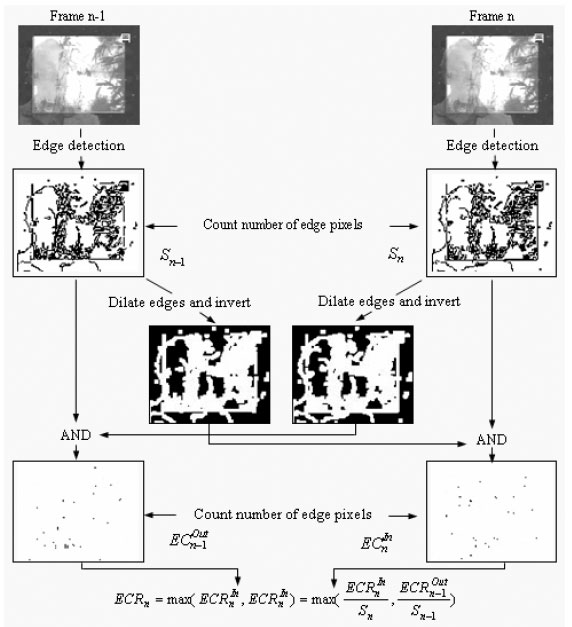
\includegraphics[width=1.0\textwidth]{fig2}
        \caption{Calculation graph of the Edge Change Ratio~\cite{ecr}}
        \label{Edge Change Ratio}
    \end{figure}
    \item Thresholds for classifying continuity: Finally, we must determine at what value of $d_i$ indicates that $f_i$ is a cut. There are many approaches to this problem, with 
    some using a local threshold, which is determined by the contextual distance values in the region of $f_i$~\cite{adaptivethresholding}, and more recently neural networks 
    have been employed to classify shots~\cite{nnthresholding}. For the purposes of this project, however, we will use a global threshold, i.e. a fixed value which when 
    exceeded by $d_i$, we consider $f_i$ to be a frame on which a cut occurs. In order to determine the optimal global threshold for each type of media, we perform performance
    tests on each piece of media and report the results on the best preforming global threshold.
\end{enumerate}
\clearpage
\subsection{Our Test Data}
We will use a BBC nature video from YouTube called "Langur monkeys grieve over fake monkey $|$ Spy in the Wild $-$ BBC" as our baseline test. The results from the 
tests on this video show how our implementations would perform on conventionally edited video. We define the frame on which a cut occurs on this video, as well as our 
other test clips from Twitch, by hand, utilizing the cut definitions described above. For our Twitch video tests, we will use clips from streamer Elajjaz playing the first 
person shooter Doom Eternal to cover our first/third person camera view, and we will use clips from streamers Zain and Mang0 playing various Super Smash Bros. games 
to test our bird's eye camera view.

\begin{figure}[ht]
    \centering
    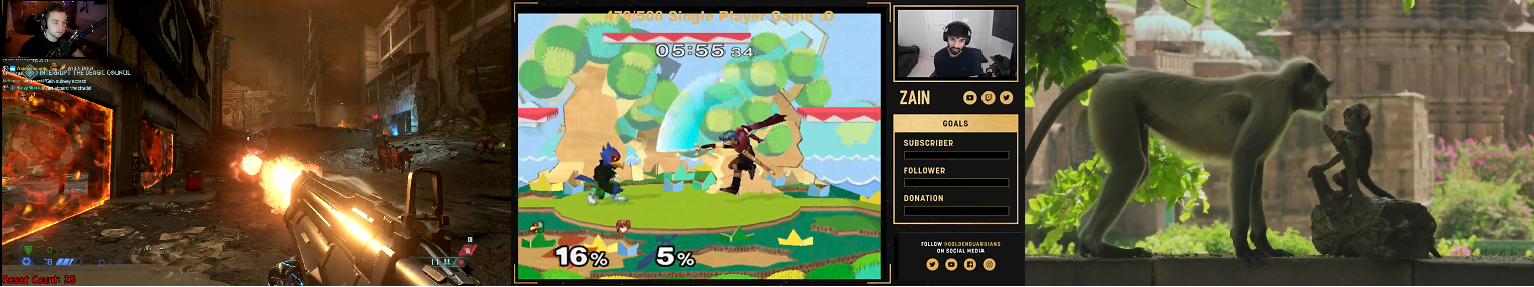
\includegraphics[width=1.0\textwidth]{fig3}
    \caption{Screenshots of our test data, From left to right: Elajjaz playing Doom Eternal, Zain playing Super Smash Bros. Melee, and Langur monkeys grieve over 
    fake monkey $|$ Spy in the Wild $-$ BBC}
    \label{Screenshots of our test data}
\end{figure}

\clearpage
\section{Results}
\subsection{Testing Results}
\begin{table}[h]
    \begin{tabular}{|l|l|l|l|}
    \hline
    Camera:                 & \multicolumn{3}{l|}{Traditional Camera Perspective}            \\ \hline
    Content Representation: & Histogram    & \multicolumn{2}{l|}{Canny Edge Detector}        \\ \hline
    Evaluation Function:    & Bhattacharya & Edge Change Ratio & SSIM \\ \hline
    Threshold(s):           & 0.3          & 0.75              & 0.75                        \\ \hline
    Recall:                 & 0.9643       & 0.8929            & 0.5                         \\ \hline
    Precision:              & 0.9310       & 0.9259            & 0.0307                      \\ \hline
    F1 Score:               & 0.9474       & 0.9091            & 0.0579                      \\ \hline
    \end{tabular}
    \caption{Traditional Camera Perspective Results}
    \label{Traditional Camera Perspective Results}
\end{table}
\begin{table}[h]
    \begin{tabular}{|l|l|l|l|l|}
    \hline
    Camera:                 & \multicolumn{4}{l|}{First/Third Person Game Camera Perspective}                   \\ \hline
    Content Representation: & \multicolumn{2}{l|}{Histogram}    & \multicolumn{2}{l|}{Canny Edge Detector} \\ \hline
    Evaluation Function:    & \multicolumn{2}{l|}{Bhattacharya} & \multicolumn{2}{l|}{Edge Change Ratio}   \\ \hline
    Threshold(s):           & 0.5, 0.15         & 0.5, 0.6      & 0.75, 0.5          & 0.75, 0.55          \\ \hline
    Recall:                 & 0.6667            & 0.3333        & 0.5000             & 0.3333              \\ \hline
    Precision:              & 0.0784            & 0.2500        & 0.25               & 0.4000              \\ \hline
    F1 Score:               & 0.1404            & 0.2857        & 0.3333             & 0.3636              \\ \hline
    \end{tabular}
    \caption{First/Third Person Game Camera Results}
    \label{First/Third Person Game Camera Results}
\end{table}
\begin{table}[h!]
    \begin{tabular}{|l|l|l|}
    \hline
    Camera:                 & \multicolumn{2}{l|}{Bird's Eye Game Camera Perpective} \\ \hline
    Content Representation: & Histogram            & Canny Edge Detector        \\ \hline
    Evaluation Function:    & Bhattacharya         & Edge Change Ratio          \\ \hline
    Threshold(s):           & 0.4, 0.6             & 0.45, 0.6                  \\ \hline
    Recall:                 & 0.8889               & 0.8889                     \\ \hline
    Precision:              & 0.8889               & 0.7273                     \\ \hline
    F1 Score:               & 0.8889               & 0.8                        \\ \hline
    \end{tabular}
    \caption{Bird's Eye Game Camera Results}
    \label{Bird's Eye Game Camera Results}
\end{table}
\subsection{Understanding the Test Results}
To be clear, the results displayed above are the abbreviated results, only showing thresholds which maximize the F1 score. For the First/Third Person Game Camera test results,
I included multiple sets of thresholds, which have differing levels of Recall and Precision, usually sacrificing Recall for increased Precision or vice versa. If there are 
multiple thresholds in a column, this is because there are multiple test sources, and each threshold corresponds to a specific video. The complete results are included in 
the submission for this project.

For our baseline testing on the Traditional Camera Perspective, we see our implementations performing quite well. As stated in previous literature ~\cite{lienhart1998comparison},
Our Canny edge detector does not outperform the simpler Colour Histogram method in the Traditional Camera Perspective. I have included the SSIM Canny Edge Detector results 
to show why this approach was discarded. Overall, these results agree with the established research; the Colour Histogram performs best for cut detection, both in F1 Score 
and in runtime speed. Our Canny edge detector was generally more sensitive to false positives in shots where there was a detailed background such as a large rock full of cracks, 
wherein subtle camera movements could detect or undetect edges in the image.

For our First/Third Person Game Camera, our implementation suffers significantly in performance. The Canny edge detector approach suffers from significant Precision problems 
due to false positives from quick camera movement, which are frequent in these types of games. Additionally, the Colour Histogram suffered from false positives from situations
where the screen would be covered by an enemy projectile. Transitions to and from the main menu were typically easy to detect, but setting the global threshold high enough to 
resist massive false positives made it extremely difficult to detect more subtle in game menu's being opened, or to detect when we more from a cutscene to gameplay, a transition
which tends to be done seamlessly to maintain the player's immersion. Overall, this type of camera perspective would benefit significantly from contextual thresholding, as the amount of false 
positives generated by global thresholds selected for their Recall performance is far too high to be useful. However, it was somewhat expected that this section would perform
poorly, as camera movement is a known false positive sensitivity for both approaches. Another more general issue solved by local thresholding is that there is no general 
global threshold that performs the best for all videos, and it can vary significantly even between games that share camera perspectives.

For our Bird's Eye Game Camera tests, our implementation performs quite well, detecting correctly most cuts and with few false positives. This result can be explained by the 
relative stability of the camera itself, significantly reducing incoming noise for both the Colour Histogram and the Canny edge detector. Additionally, cutscenes are sparse
in the genres which sport these camera perspectives, specifically fighting games and roguelikes, further reducing noise. Most of the cuts occur at the beginning and at the end 
of a match/level, which mostly falls under the main menu to gameplay transitions, which we continue to perform well in.
\subsection{Conclusion}
Overall, this project has outlined the practicality of the shot boundary detection problem for video game live streaming, and has 
shown a promising proof of concept for cut detection for streamers who play games with a Bird's Eye camera perspective, such as fighting games or 
roguelikes. In order to improve performance for more dynamic camera perspectives, local thresholding and noise reduction strategies would likely improve performance.
\clearpage

\bibliography{mybib}{}
\bibliographystyle{apalike}
\clearpage

\end{document}